



\section{Neural Networks}
%
\subsection{Introduction}
%
\begin{frame}[t]{What is a neural network?}
A neural network is a model that learns how to map fingerprints (in this case, of a molecule) to output quantities (atomization energies, spin-splitting energies).
\visible<2->{\par Nonlinear activation functions make neural networks powerful.}
\visible<3->{\par $\sigma(z)\rightarrow ReLU(z)=$\[ \begin{cases} 
z & z>0 \\
0 & otherwise
\end{cases}
\]}
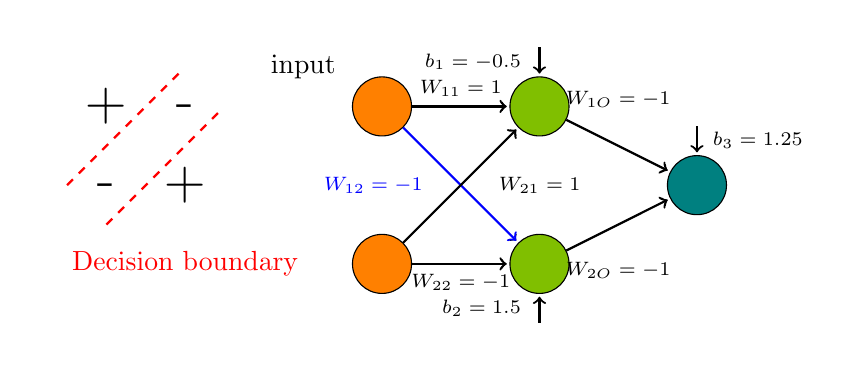
\begin{tikzpicture}[shorten >=1pt,draw=black, x=1cm, y=1 cm,  node distance=0cm]
	\draw[draw=none, use as bounding box](-2,0) rectangle (8,4);
	\clip (-2,-0) rectangle (8,6);
	\def\layersep{2cm}
	
    \tikzstyle{every pin edge}=[<-,shorten <=1pt,thick]
    \tikzstyle{neuron}=[circle,fill=black!25,minimum size=0.75cm ,inner sep=0pt, color=black, draw]
    \tikzstyle{input neuron}=[neuron, fill=green!50!blue!50];
    \tikzstyle{output neuron}=[neuron, fill=green!50!blue];
    \tikzstyle{hidden neuron}=[neuron, fill=green!50!orange];
    \tikzstyle{annot} = [text width=2em, text centered]
    \visible<4->{\node[] (I) at (-1,2) {\huge-};}
    \visible<4->{\node[] (I) at (-1,3) {\huge+};}
    \visible<4->{\node[] (I) at (0,2) {\huge+};}
    \visible<4->{\node[] (I) at (0,3) {\huge-};}
    \visible<5->{\draw[red,thick,dashed] (-1.5,2) -- (0,3.5);}
    \visible<5->{\draw[red,thick,dashed] (-1,1.5) -- (0.5,3);}
    \visible<5->{\node[red] (I) at (0,1) {Decision boundary};}
	\visible<6->{\node[](l) at (1.5, 3.5) {input};}
	\visible<6->{\node[input neuron,fill=orange!100 ] (I-1) at (2.5,1) {$ $};}
	\visible<6->{\node[input neuron,fill=orange!100 ] (I-2) at (2.5,3) {$ $};}
	\visible<6->{\node[hidden neuron,fill=green!50!orange] (H-1) at (4.5,1) {$ $};}
	\visible<6->{\node[hidden neuron,fill=green!50!orange] (H-2) at (4.5,3) {$ $};}
	\visible<6->{\node[output neuron,fill=green!50!blue] (O) at (6.5,2) {$ $};}
	\foreach \dest in {1,2}{     
		\foreach \source in {1,2}{
			\visible<6->{\path[thin,->,black] (I-\source) edge node[font=\scriptsize] {} (H-\dest) ;}}
		}
	\visible<6->{\path[thin,->,black] (H-1) edge node[font=\scriptsize] {} (O);}
	\visible<6->{\path[thin,->,black] (H-2) edge node[font=\scriptsize] {} (O);}
	\visible<7->{\path[thick,->,black, midway, above,black] (I-2) edge node[font=\scriptsize] {$W_{11}=1$} (H-2) ;}
	\visible<7->{\path[thick,->,blue, midway, left,blue] (I-2) edge node[font=\scriptsize, left=10pt] {$W_{12}=-1$} (H-1) ;}
	\visible<7->{\path[thick,->,black, midway, right,black] (I-1) edge node[font=\scriptsize, right=10pt] {$W_{21}=1$} (H-2) ;}
	\visible<7->{\path[thick,->,black, midway, below,black] (I-1) edge node[font=\scriptsize] {$W_{22}=-1$} (H-1) ;}
	\visible<7->{\path[thick,->,black, midway, below,black] (H-1) edge node[font=\scriptsize, below = 10pt] {$W_{2O}=-1$} (O) ;}
	\visible<7->{\path[thick,->,black, midway, below,black] (H-2) edge node[font=\scriptsize, above = 10pt] {$W_{1O}=-1$} (O) ;}
	\visible<7->{\path[thick,->,black, midway, below,black] (4.5,0.25) edge node[font=\scriptsize, left = 3pt] {$b_2=1.5$} (H-1) ;}
	\visible<7->{\path[thick,->,black, midway, below,black] (4.5,3.75) edge node[font=\scriptsize, left = 3pt] {$b_1=-0.5$} (H-2) ;}
	\visible<7->{\path[thick,->,black, midway, below,black] (6.5,2.75) edge node[font=\scriptsize, right = 2pt] {$b_3=1.25$} (O) ;}
\end{tikzpicture}

\end{frame}
%
\subsection{Mechanics}
%
\begin{frame}[t]{The neuron}
\begin{tikzpicture}[shorten >=1pt,draw=black, x=1cm, y=1 cm,  node distance=0cm]

\draw[use as bounding box, anchor = north west,draw=none] (-2,-4.25) rectangle (9,3.25);
\clip (-2,-4.25) rectangle (9.0,3.25);

%% setup parameters for NN drawing

\tikzstyle{every pin edge}=[<-,shorten <=1pt,thick]
\tikzstyle{neuron}=[circle,fill=black!25,minimum size=0.75cm ,inner sep=0pt, color=black, draw]
\tikzstyle{input neuron}=[neuron, fill=green!25!blue!25];
\tikzstyle{output neuron}=[neuron, fill=green!25!blue!50];
\tikzstyle{hidden neuron}=[neuron, fill=green!50!orange!25];
\tikzstyle{annot} = [text width=2cm, text centered]


%% define coordinate grid 
\def \xfarleft {-1.25}
\def \xleft {-1.0}
\def \xmid {-0.25}
\def \xright {0.5}
\def \ytop {1.0}
\def \ymid {-0.5}
\def \ybot {-1.15}
\def \yphasetwo {-2.0}
\def \xlabeloffset {0.05}
\def \ylabeloffset {0.15}
\def\layersep{3.0}
\def\vlayersep{1.5}



% Draw the input layer nodes
\visible<2->{\node  (ll) at (\xfarleft,\ymid+1.5*\vlayersep) {\small inputs};}
\visible<2->{\node  (ll) at (\xfarleft,\ymid-1.5*\vlayersep) {$x\in\mathbb{R}^{1\times 3}$};}
\foreach \name/\y in {1/\ymid-\vlayersep,2/\ymid,3/\ymid+\vlayersep}{
\visible<2->{\node[input neuron,fill=orange!100 ] (I-\name) at (\xfarleft,\y) {$I_{\name}$};}
}





\foreach \name/\y in {1/\ymid}{
\visible<2->{\path node[hidden neuron] (H-\name) at (\xfarleft+\layersep,\y) {$\sigma$};}
}



% Draw the output layer node
\visible<2->{\node[thick, output neuron] at (\xfarleft+2.0*\layersep,\ymid) (O) {$O$};}



\foreach \source in {1}{
	\visible<2->{\path[thick,->,black] (H-\source) -- (O) ;}}

\visible<2->{\path[thick,->,black,draw] (O.east) -- ([xshift=0.25*\layersep cm]O.east);}

\visible<2->{\node [anchor=west] (l2) at ([xshift=0.25*\layersep cm]O.east) {\small property};}


\foreach \source in {1}{
	\visible<2->{\path[->,black,draw,thick] (H-\source) -- (O) ;}}

\foreach \source in {1}{
		\visible<4->{\path[thick,->,blue] (H-\source) edge node[rectangle, fill=white,fill opacity=0.75,text opacity=1] {$\color{black}\sigma\left(x{\color{blue}w}\right)$} (O) ;}}



\visible<5>{\node[anchor= west, draw, gray,very thick,fill=white] (latt) at (\xmid+4.5,\ymid) {{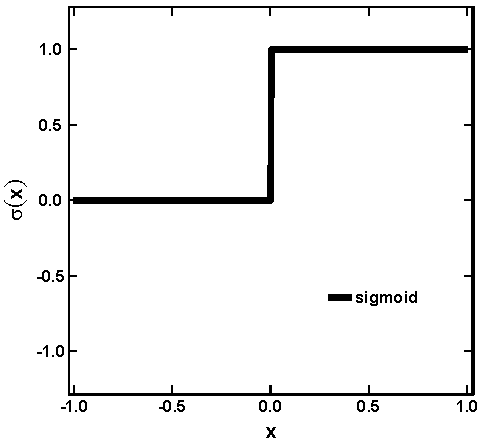
\includegraphics[width= 4.0 cm]{neural_networks/images/act_1}}};}
\visible<6>{\node[anchor= west, draw, gray,very thick,fill=white] (latt) at (\xmid+4.5,\ymid) {{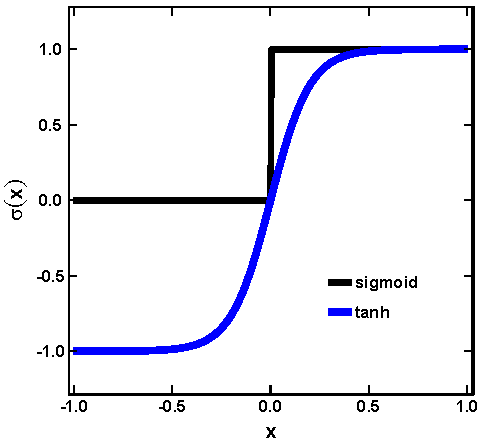
\includegraphics[width= 4.0 cm]{neural_networks/images/act_2}}};}
\visible<7>{\node[anchor= west, draw, gray,very thick,fill=white] (latt) at (\xmid+4.5,\ymid) {{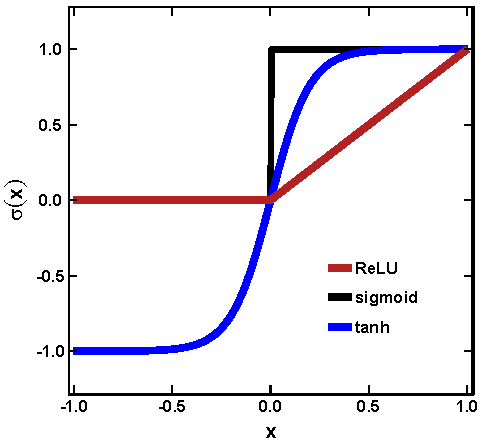
\includegraphics[width= 4.0 cm]{neural_networks/images/act_3}}};}
%
\node[anchor = north west] at (\xmid+1,\ymid-2.0) {
\begin{minipage}{8cm}
\visible<5->{This unit is differentiable as long as $\sigma$ is.}
\vspace{-0.25cm}
\begin{align*}
\only<6>{\frac{\partial O}{\partial {\color{blue}w_1}}&=x_1\sigma'\left(x{\color{blue}w}\right)}
\only<7->{\implies \frac{\partial O}{\partial {\color{blue}w}}  &= x\sigma'\left(x{\color{blue}w}\right)}
\end{align*}
\end{minipage}};
%
%\node[anchor = north west] at (\xmid+0.5,\ymid+2.75) {
%\begin{minipage}{8cm}
%\visible<8->{Note: we do not change anything about $\sigma$, we only tweak the linear combinations of inputs.}
%\end{minipage}};



\foreach \source in {1,2,3}{
\foreach \dest in {1}{     

\visible<2->{\path[thick,->,black] (I-\source) edge[thick] node[] {} (H-\dest) ;}}
}


\foreach \source in {1,2,3}{
\foreach \dest in {1}{     
\visible<3->{\path[thick,->,blue] (I-\source) edge node[rectangle, fill=white,fill opacity=0.5,opacity=1] {{\color{blue}$w_{\source}$}{\color{black}$x_{\source}$}} (H-\dest) ;}}
}




\end{tikzpicture}


\end{frame}
%
\begin{frame}[t]{The perceptron}
\begin{tikzpicture}[shorten >=1pt,draw=black, x=1cm, y=1 cm,  node distance=0cm]

\draw[use as bounding box, anchor = north west,draw=none] (-2,-4.25) rectangle (9,3.25);
\clip (-2,-4.25) rectangle (9.0,3.25);

%% setup parameters for NN drawing

\tikzstyle{every pin edge}=[<-,shorten <=1pt,thick]
\tikzstyle{neuron}=[circle,fill=black!25,minimum size=0.75cm ,inner sep=0pt, color=black, draw]
\tikzstyle{input neuron}=[neuron, fill=green!25!blue!25];
\tikzstyle{output neuron}=[neuron, fill=green!25!blue!50];
\tikzstyle{hidden neuron}=[neuron, fill=green!50!orange!25];
\tikzstyle{annot} = [text width=2cm, text centered]


%% define coordinate grid 
\def \xfarleft {-1.25}
\def \xleft {-1.0}
\def \xmid {-0.25}
\def \xright {0.5}
\def \ytop {1.0}
\def \ymid {-0.5}
\def \ybot {-1.15}
\def \yh {3.25}
\def \yphasetwo {-2.0}
\def \xlabeloffset {0.05}
\def \ylabeloffset {0.15}
\def\layersep{3.0}
\def\vlayersep{1.5}

% Draw the input layer nodes
\visible<1->{\node  (ll) at (\xfarleft,\ymid+1.5*\vlayersep) {\small inputs};}
\visible<2->{\node  (ll) at (\xfarleft,\ymid-1.5*\vlayersep) {$x\in\mathbb{R}^{1\times 3}$};}
\visible<2->{\node  (ll) at (\xfarleft+\layersep,\ymid-2.0*\vlayersep) {$z\in\mathbb{R}^{1\times 4}$};}

\foreach \name/\y in {1/\ymid-\vlayersep,2/\ymid,3/\ymid+\vlayersep}{
\visible<1->{\node[input neuron,fill=orange!100 ] (I-\name) at (\xfarleft,\y) {$I_{\name}$};}
}

% Draw the hidden layer nodes

\foreach \name/\y in {1/\ymid}{
\visible<1>{\path node[hidden neuron] (H-\name) at (\xfarleft+\layersep,\y) {$\sigma$};}
}

\foreach \name/\y in {1/\ymid-1.5*\vlayersep,
	2/\ymid-0.5*\vlayersep,
	3/\ymid+0.5*\vlayersep,
	4/\ymid+1.5*\vlayersep}{
\only<2->{\path node[hidden neuron] (H-\name) at (\xfarleft+\layersep,\y) {$H_{1,\name}$};}
}



% Draw the output layer node
\visible<1->{\node[thick, output neuron] at (\xfarleft+2*\layersep,\ymid) (O) {$O$};}




\foreach \source in {1}{
\visible<1->{\path[thick,->,black] (H-\source) -- (O) ;}}

\visible<1->{\path[thick,->,black,draw] (O.east) -- ([xshift=0.25*\layersep cm]O.east);}

\visible<1->{\node [anchor=west] (l2) at ([xshift=0.25*\layersep cm]O.east) {\small property};}


\foreach \source in {1}{
\only<1>{\path[->,black,draw,thick] (H-\source) -- (O) ;}}

\foreach \source in {1,2,3,4}{
\only<2-4>{\path[->,black,draw,thick] (H-\source) -- (O) ;}}

\foreach \source in {1,2,3,4}{
%\only<4->{\path[->,gray,draw,thick,opacity=0.5] (H-\source) -- (O) ;}}
\only<5->{\path[thick,->,blue] (H-\source) edge node[rectangle, fill=white,fill opacity=0.75,text opacity=1] {{\color{blue}$w_{\source,1}^1$}{\color{black}$z_{\source}$}} (O) ;}}



%\foreach \source in {1}{
%\visible<4->{\path[thick,->,blue] (H-\source) edge node[rectangle, fill=white,fill opacity=0.5,opacity=1] {\color{blue}$\sigma\left(w^Tx\right)$} (O) ;}}

\visible<3-4>{\node[anchor = north west] at (\xmid+1.75,\ymid-0.5) {
\begin{minipage}{8cm}
\small
\begin{align*}
z=\begin{bmatrix}
\sigma \left(x {\color{blue}w_{:,1}^0} \right)\\
\sigma \left(x {\color{blue}w_{:,2}^0} \right)\\
\sigma \left(x {\color{blue}w_{:,3}^0} \right)\\
\sigma \left(x {\color{blue}w_{:,4}^0} \right)\\
\end{bmatrix}^T
=&\sigma\left(x{\color{blue}W^0}\right)\\
\visible<4>{&\color{blue}W^0\color{black}\in\mathbb{R}^{3\times4}}
\end{align*}
\end{minipage}};}

\visible<5->{\node[anchor = north west] at (\xmid+1.75,\ymid-0.5) {
\begin{minipage}{8cm}
\small
\begin{align*}
O&=z{\color{blue}w^1} =\sigma\left(x {\color{blue}W^0} \right){\color{blue}w^1}\\
\only<6-7>{\textrm{c.f. } \hat{y}&= \varphi(x)w\\}
\only<8->{\frac{\partial O}{\partial {\color{blue}w_{1,1}^{0}}}&=\party{z}{\color{blue}w_{1,1}^{0}}{\color{blue}w^1}\\}
\only<9->{&=x_1\sigma'\left(x{\color{blue} W^0} \right){\color{blue}w^1}}
\end{align*}
\end{minipage}};}

\node[anchor = north west] at (\xmid+4,\ymid+2.75) {
\begin{minipage}{7cm}
\visible<7>{\textbf{What is} $k(x,x^*)$ \textbf{here?}}
\end{minipage}};

%\foreach \source in {1,2,3,4}{
%	{\path[thick,->,blue] (H-\source) edge node[rectangle, fill=white,fill opacity=0.5,opacity=1] {\color{blue}$w_{\source,1}^{1}$} (O) ;}}


%\foreach \source in {1,2,3,4}{
%	{\path[thick,->,blue] (H-\source) edge node[rectangle, fill=white,fill opacity=0.5,opacity=1] {\color{blue}$w_{\source,1}^{1}$} (O) ;}}


%\foreach \source in {1,2,3}{
%\foreach \dest in {}{     
%	\path[thick,->,gray,opacity=0.5] (I-\source) edge node[] {} (H-\dest) ;}}


% input to H 1st
\foreach \source in {1,2,3}{
\foreach \dest in {1}{     
\only<1>{\path[thick,->,black] (I-\source) edge[thick] node[] {} (H-\dest) ;}}
}

% input to H 2nd
\foreach \source in {1,2,3}{
\foreach \dest in {1,2,3,4}{     
\only<2>{\path[thick,->,black] (I-\source) edge[thick] node[] {} (H-\dest) ;}}
}

% input to H 3rd
\foreach \source in {2,3}{
	\foreach \dest in {1,2,3,4}{     
		\only<3->{\path[thick,->,gray, opacity=0.5] (I-\source) edge[thick] node[] {} (H-\dest) ;}}
}


\foreach \source in {1}{
\foreach \dest in {4,3,2,1}{     
\only<3->{\path[thick,->,blue] (I-\source) edge node[rectangle, fill=white,fill opacity=0.75,text opacity=1] {{\color{blue}$w_{\source,\dest}^0$}{\color{black}$x_{\source}$}} (H-\dest) ;}}
}




\end{tikzpicture}


\end{frame}
%
\begin{frame}[t]{The \textit{multilayer} perceptron}
\begin{tikzpicture}[shorten >=1pt,draw=black, x=1cm, y=1 cm,  node distance=0cm]

\draw[use as bounding box, anchor = north west,draw=none] (-2,-4.25) rectangle (9,3.25);
\clip (-2,-4.25) rectangle (9.0,3.25);

%% setup parameters for NN drawing

\tikzstyle{every pin edge}=[<-,shorten <=1pt,thick]
\tikzstyle{neuron}=[circle,fill=black!25,minimum size=0.75cm ,inner sep=0pt, color=black, draw]
\tikzstyle{input neuron}=[neuron, fill=green!25!blue!25];
\tikzstyle{output neuron}=[neuron, fill=green!25!blue!50];
\tikzstyle{hidden neuron}=[neuron, fill=green!50!orange!25];
\tikzstyle{annot} = [text width=2cm, text centered]


%% define coordinate grid 
\def \xfarleft {-1.25}
\def \xleft {-1.0}
\def \xmid {-0.25}
\def \xright {0.5}
\def \ytop {1.0}
\def \yh {3.25}
\def \ymid {-0.5}
\def \ybot {-1.15}
\def \yphasetwo {-2.0}
\def \xlabeloffset {0.05}
\def \ylabeloffset {0.15}
\def\layersep{3.0}
\def\vlayersep{1.5}

% Draw the input layer nodes
\visible<1->{\node  (ll) at (\xfarleft,\ymid+1.5*\vlayersep) {\small inputs};}
\visible<1->{\node  (ll) at (\xfarleft,\ymid-1.5*\vlayersep) {$x\in\mathbb{R}^{1\times 3}$};}
\visible<1>{\node  (ll) at (\xfarleft+\layersep,\ymid-2.0*\vlayersep) {$z\in\mathbb{R}^{1\times 4}$};}
\visible<2->{\node  (ll) at (\xfarleft+\layersep,\ymid-2.0*\vlayersep) {$z^1\in\mathbb{R}^{1\times 4}$};}
\visible<2->{\node  (ll) at (\xfarleft+2*\layersep,\ymid-2.0*\vlayersep) {$z^2\in\mathbb{R}^{1\times 4}$};}

\foreach \name/\y in {1/\ymid-\vlayersep,2/\ymid,3/\ymid+\vlayersep}{
\visible<1->{\node[input neuron,fill=orange!100 ] (I-\name) at (\xfarleft,\y) {$I_{\name}$};}
}

% Draw the hidden layer nodes


\foreach \name/\y in {1/\ymid-1.5*\vlayersep,
	2/\ymid-0.5*\vlayersep,
	3/\ymid+0.5*\vlayersep,
	4/\ymid+1.5*\vlayersep}{
\only<1->{\path node[hidden neuron] (H-\name) at (\xfarleft+\layersep,\y) {$H_{1,\name}$};}
\only<2->{\path node[hidden neuron] (H2-\name) at (\xfarleft+2*\layersep,\y) {$H_{2,\name}$};}
}



% Draw the output layer node
\only<1>{\node[thick, output neuron] at (\xfarleft+2*\layersep,\ymid) (O) {$O$};}
\only<2->{\node[thick, output neuron] at (\xfarleft+3*\layersep,\ymid) (O) {$O$};}

\visible<1->{\path[thick,->,black,draw] (O.east) -- ([xshift=0.25*\layersep cm]O.east);}

\only<1>{\node [anchor=west] (l2) at ([xshift=0.25*\layersep cm]O.east) {\small property};}




\foreach \source in {1,2,3,4}{
\only<1>{\path[->,black,draw,thick] (H-\source) -- (O) ;}
\only<2-4>{\path[->,black,draw,thick] (H2-\source) -- (O) ;}
}

\foreach \source in {1,2,3,4}{
\only<5->{\path[thick,->,blue] (H2-\source) edge node[rectangle, fill=white,fill opacity=0.75,text opacity=1] {{\color{blue}$w_{\source,1}^2$}{\color{black}$z_{\source}^2$}} (O) ;}}



%\foreach \source in {1}{
%\visible<4->{\path[thick,->,blue] (H-\source) edge node[rectangle, fill=white,fill opacity=0.5,opacity=1] {\color{blue}$\sigma\left(w^Tx\right)$} (O) ;}}


%\visible<5->{\node[anchor = north west] at (\xmid+1.75,\ymid-1.0) {
%\begin{minipage}{8cm}
%\small
%\begin{align*}
%O&=z{\color{blue}w^1} =\sigma\left(W^0 x\right){\color{blue}w^1}\\
%\visible<6->{\textrm{c.f. } \hat{y}&= \varphi(x)w}
%\end{align*}
%\end{minipage}};}

%\node[anchor = north west] at (\xmid+4,\ymid+2.75) {
%\begin{minipage}{7cm}
%\visible<7->{What is $k(x,x^*)$ here?}
%\end{minipage}};

%\foreach \source in {1,2,3,4}{
%	{\path[thick,->,blue] (H-\source) edge node[rectangle, fill=white,fill opacity=0.5,opacity=1] {\color{blue}$w_{\source,1}^{1}$} (O) ;}}


%\foreach \source in {1,2,3,4}{
%	{\path[thick,->,blue] (H-\source) edge node[rectangle, fill=white,fill opacity=0.5,opacity=1] {\color{blue}$w_{\source,1}^{1}$} (O) ;}}


%\foreach \source in {1,2,3}{
%\foreach \dest in {}{     
%	\path[thick,->,gray,opacity=0.5] (I-\source) edge node[] {} (H-\dest) ;}}



% input to H 1st
\foreach \source in {1,2,3}{
\foreach \dest in {1,2,3,4}{     
\only<1-2>{\path[thick,->,black] (I-\source) edge[thick] node[] {} (H-\dest) ;}
\only<3->{\path[thick,->,black,gray,opacity=0.5] (I-\source) edge[thick] node[] {} (H-\dest) ;}
}
}


\foreach \source in {1,2,3,4}{
\foreach \dest in {1,2,3,4}{     
\only<2-3>{\path[thick,->,black] (H-\source) edge[thick] node[] {} (H2-\dest) ;}
\only<4->{\path[thick,->,gray, opacity=0.5] (H-\source) edge[thick] node[] {} (H2-\dest) ;}
}
}

% input to H 3rd
%\foreach \source in {2,3}{
%	\foreach \dest in {1,2,3,4}{     
%		\only<3->{\path[thick,->,gray, opacity=0.5] (I-\source) edge[thick] node[] {} (H-\dest) ;}}
%}


%% colored I-H1
\foreach \source in {1,2,3}{
\foreach \dest in {1}{     
\only<3->{\path[thick,->,blue] (I-\source) edge node[rectangle, fill=white,fill opacity=0.75,text opacity=1] {{\color{blue}$w_{\source,\dest}^0$}{\color{black}$x_{\source}$}} (H-\dest) ;}}
}

%% colored H1-H2
\foreach \source in {1}{
\foreach \dest in {1,2,3,4}{     
\only<4->{\path[thick,->,blue] (H-\source) edge node[rectangle, fill=white,fill opacity=0.75,text opacity=1] {{\color{blue}$w_{\source,\dest}^1$}{\color{black}$z_{\source}^{1}$}} (H2-\dest) ;}}
}

\visible<6->{\node[anchor = north west,fill=white, opacity=1.0,text opacity=1,draw = gray] at (\xmid-1.75,\yh) {
		\begin{minipage}{8cm}
		\small
		\begin{align*}
		O&=z^2{\color{blue}w^2} =\sigma\left(z^1 {\color{blue} W^1} \right){\color{blue}w^2} \\
		\only<7->{&= \sigma\left(\left[\sigma\left(x {\color{blue} W^0}\right)\right] {\color{blue} W^1} \right){\color{blue}w^2}\\}
		\only<8->{\frac{\partial O}{\partial {\color{blue}w_{1,1}^{0}}}&=\party{z^2}{\color{blue}w_{1,1}^{0}}{\color{blue}w^2} 
		\visible<9->{=\party{z^1}{\color{blue} w_{1,1}^{0}} \sigma'\left(z^1 {\color{blue} W^1} \right){\color{blue}w^2}}\\}
		\only<10->{&= x_1\sigma'\left(x{\color{blue} W^0} \right)\sigma'\left(z^1 {\color{blue} W^1} \right){\color{blue}w^2}}
		\end{align*}
		\only<11->{This is called \textbf{back propagation}.}
		\end{minipage}};}

\end{tikzpicture}


\end{frame}
%
\begin{frame}[t]\frametitle{How ANNs work}

\begin{tikzpicture}[x=1cm, y=1cm]
\def\xstart{-2.5}
\def\xend{8.5}
\def\ystart{1.0}
\def\yend{8}
\draw[use as bounding box, anchor = north west,draw=none] (\xstart,\ystart) rectangle (\xend,\yend);
\clip (\xstart-0.5,\ystart-0.5) rectangle (\xend+0.5,\yend+0.5);
%%% get train data
%\visible<4->{\node[rectangle,very thick,opacity = 0.15,fill=red,red,minimum width = 1.5cm, minimum height = 1.5cm, label=above:{\color{red}{few training points}}] (ci) at (1.5,3.5){};}

\def\layersep{1.05}
\def\vlayersep{0.6}

\tikzstyle{every pin edge}=[<-,shorten <=1pt,thick]
\tikzstyle{neuron}=[circle,fill=black!25,minimum size=0.3cm ,inner sep=0pt, color=black, draw]
\tikzstyle{input neuron}=[neuron, fill=green!50!blue!50];
\tikzstyle{output neuron}=[neuron, fill=green!50!blue];
\tikzstyle{hidden neuron}=[neuron, fill=green!50!orange];
\tikzstyle{annot} = [text width=2cm, text centered]
% tsnes
\visible<3->{\node[anchor=south] (ract) at (0.5,3.15) {{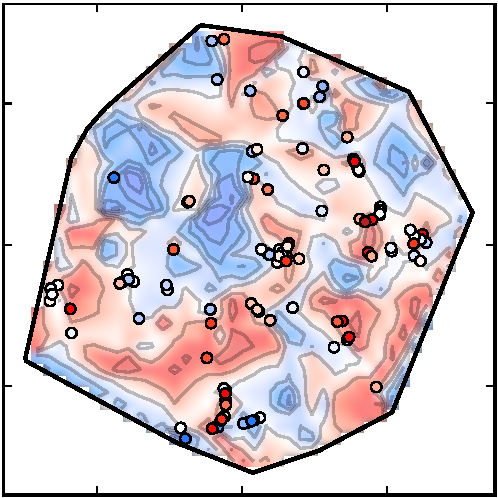
\includegraphics[width= 4.0cm]{neural_networks/images/talk-rac-tsne-t-n}}};}
\visible<9->{\node[anchor=south] (latt) at (5.5,3.15) {{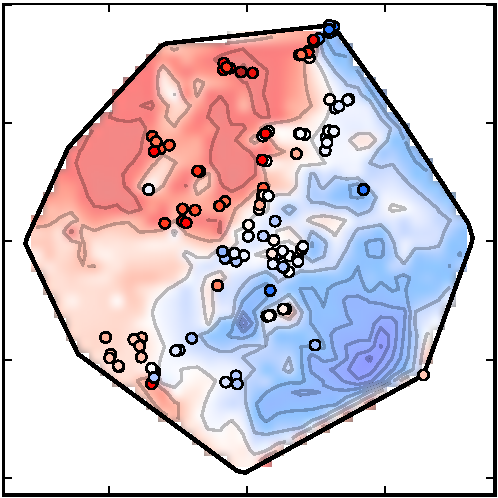
\includegraphics[width= 4.0cm]{neural_networks/images/talk-lat-tsne-t-n}}};}


\def\xof{0.25}
\def\xwd{0.20}
\def\arw{0.10}
\begin{scope}[shift={(0,-0.25)}]
\visible<3->{\draw [black,->,thick, fill=orange] (1.125,3) to [bend left] 
(\xof,3.75) -- (\xof-\arw,3.75) -- (\xof+0.5*\xwd,4.0) -- (\xwd+\xof+\arw,3.75) -- (\xof+\xwd,3.75) to [bend right] (1.125,3.20) --cycle;}
\end{scope}



\def\xof{5.775}
\def\xwd{0.20}
\def\arw{0.10}
\begin{scope}[shift={(0,-0.25)}]
\visible<9->{\draw [black,->,thick, fill=green!50!orange] (4.90,3) to [bend right] 
(\xof+\xwd,3.75)  -- (\xwd+\xof+\arw,3.75)  -- (\xof+0.5*\xwd,4.0) --(\xof-\arw,3.75) -- (\xof,3.75) to [bend left] (4.90,3.20) --cycle;}
\end{scope}
\begin{scope}[shift={(3-1.5*\layersep,-0.5)}]
% draw callout planes
\visible<2->{\node[rectangle, draw, fill=orange, fill opacity=0.15,color=orange, thick,
minimum height = 2.85*\vlayersep cm, minimum width=0.5cm] at (0,3){};}
\visible<8->{\node[rectangle, draw, fill=green!50!orange, fill opacity=0.15,color=green!50!orange, thick,
minimum height = 3.75*\vlayersep cm, minimum width=0.5cm] at (3*\layersep,3){}; }


% Draw the input layer nodes
\foreach \name/\y in {1/3-\vlayersep,2/3,3/3+\vlayersep}{
\visible<2->{\node[input neuron,fill=orange!100 ] (I-\name) at (0,\y) {$ $};}}

% Draw the hidden layer nodes
\foreach \name/\y in {1/3-1.5*\vlayersep,2/3-0.5*\vlayersep,3/3+0.5*\vlayersep,4/3+1.5*\vlayersep}{
	\visible<4->{\path[yshift=0.5] node[hidden neuron] (H-\name) at (\layersep,\y) {\small $ $};}
	\visible<5->{\path[yshift=0.5] node[hidden neuron] (H2-\name) at (2*\layersep,\y) {\small $ $};}
	\visible<6->{\path[yshift=0.5] node[hidden neuron] (H3-\name) at (3*\layersep,\y) {\small $ $};}
}
% Draw the output layer node
\visible<7->{\node[thin, output neuron,pin={[pin edge={->}]right:\footnotesize }] at (3.5*\layersep,3) (O) {$ $};}

\foreach \dest in {1,2,3,4}     
\foreach \source in {1,2,3,4}
{
	\visible<5->{\path[thin,->] (H-\source) edge node[font=\scriptsize] {} (H2-\dest) ;}
	\visible<6->{\path[thin,->] (H2-\source) edge node[font=\scriptsize] {} (H3-\dest) ;}
}

\foreach \source in {1,2,3,4}{
	\visible<7->{\path[thin,->] (H3-\source) edge node[font=\scriptsize] {} (O) ;}}
\foreach \source in {1,2,3}
\foreach \dest in {1,2,3,4}{     
	\visible<4->{\path[thin,->] (I-\source) edge node[font=\scriptsize] {} (H-\dest) ;}}


\visible<2->{
\node[circle, black,thick,minimum width = 2.7cm,minimum height = 2.7cm,path picture={\node at (path picture bounding box.center){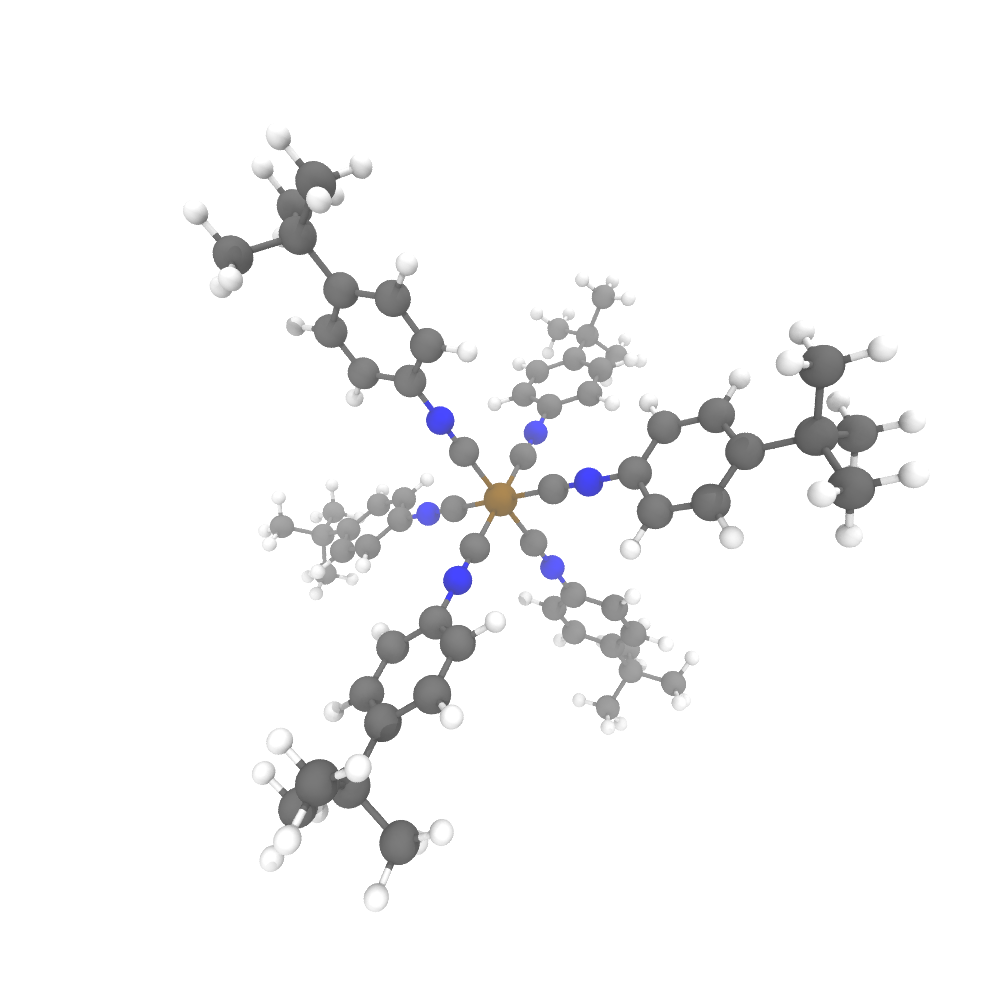
\includegraphics[width=3cm]{representations/images/pisc_trans}}; }] (Xp) at (-2.75,4) {};}

\visible<2->{\node [rotate=0] (ll) at (-1.5,3) {\small input molecule};}
\visible<7->{\node [rotate=0] (l2) at (5.25,3) {\small property};}
\end{scope}	               

%% pane lables
\visible<1->{\node [anchor=south west, text width = 12cm] (la) at (-2.5,7.75) {\small ANNs learn nonlinear reorganizations of the input to make prediciton easier:};}
\visible<3-9>{\node [anchor=south west] (la) at (-1.75,7.25) {\small \textbf{feature space}};}
\visible<9->{\node [anchor=south west] (lb) at (-1.75+5,7.25) {\small \textbf{latent space}};}



\end{tikzpicture}




\end{frame}
%
\begin{frame}[t]{SGD and training process}
\visible<1->{Backpropagation is normally used to find the gradients. Since all of the gradients are made easy to find with backpropagation, they can be updated with gradient descent:}
\visible<2->{$$W = W-\eta *\Big(\frac{\partial Loss}{\partial W}\Big)$$}
\visible<3->{In gradient descent, loss term calculated from training data $\rightarrow$ if you train for the same number of epochs (number of rounds your NN sees the training data), you will get the same result. \textbf{Gets stuck in local minima!}}
\visible<4->{$$GD\rightarrow\Big(\frac{\partial Loss}{\partial W}\Big)\rightarrow all\:training\:data$$}
\visible<5->{$$SGD\rightarrow\Big(\frac{\partial Loss}{\partial W}\Big)\rightarrow one/few\:examples\rightarrow MUCH\:noisier!\rightarrow less\:stuck$$}
\end{frame}
%
\begin{frame}[t]{Other types of layers}
\visible<1->{\textbf{Input}$\rightarrow$ layers on the NN where inputs are fed}\\
\visible<2->{\textbf{Hidden}$\rightarrow$ layers between the input and output nodes, helps to create the latent space (rearrangement of initial input points in space)}\\
\visible<3->{\textbf{Dropout}$\rightarrow$ zero out nodes to reduce specific node dependence\\
\visible<4->\textbf{Output}$\rightarrow$ Node right before result, linear for regression, sigmoid for classification. Maps latent space to final answer}\\
\visible<5->{\textbf{Convolutional}$\rightarrow$ Layer used to extract information or ``focus on" certain features. Use a sliding ``feature detector" called a filter, which creates a map}\\
\visible<6->{\textbf{Recurrent}$\rightarrow$ Layers that ``store" information about previous times, thus commonly used in speech or handwriting recognition}
\end{frame}
%
\subsection{Representation learning}
%
\begin{frame}[t]{Interpretation as representation learning}
\visible<1->{A neural network (NN) takes an initial representation as an input.}\\
\visible<2->{Hidden layers in the NN utilize distort the representation in a high dimensional space, thus learning a new representation. This separation allows ease of classification or regression}\\
\begin{tikzpicture}[shorten >=1pt,draw=black, x=1cm, y=1 cm,  node distance=0cm]
	\draw[draw=gray, use as bounding box](-2,0) rectangle (8,6);
	\clip (-2,-0) rectangle (8,6);
	\def\layersep{2cm}
	
	\tikzstyle{every pin edge}=[<-,shorten <=1pt,thick]
	\tikzstyle{neuron}=[circle,fill=black!25,minimum size=0.5cm ,inner sep=0pt, color=black, draw]
	\tikzstyle{input neuron}=[neuron, fill=green!50!blue!50];
	\tikzstyle{output neuron}=[neuron, fill=green!50!blue];
	\tikzstyle{hidden neuron}=[neuron, fill=green!50!orange];
	\tikzstyle{annot} = [text width=2em, text centered]

	\visible<3->{\node[black,thick,minimum width = 8cm,minimum height = 8cm,path picture={\node at (path picture bounding box.center){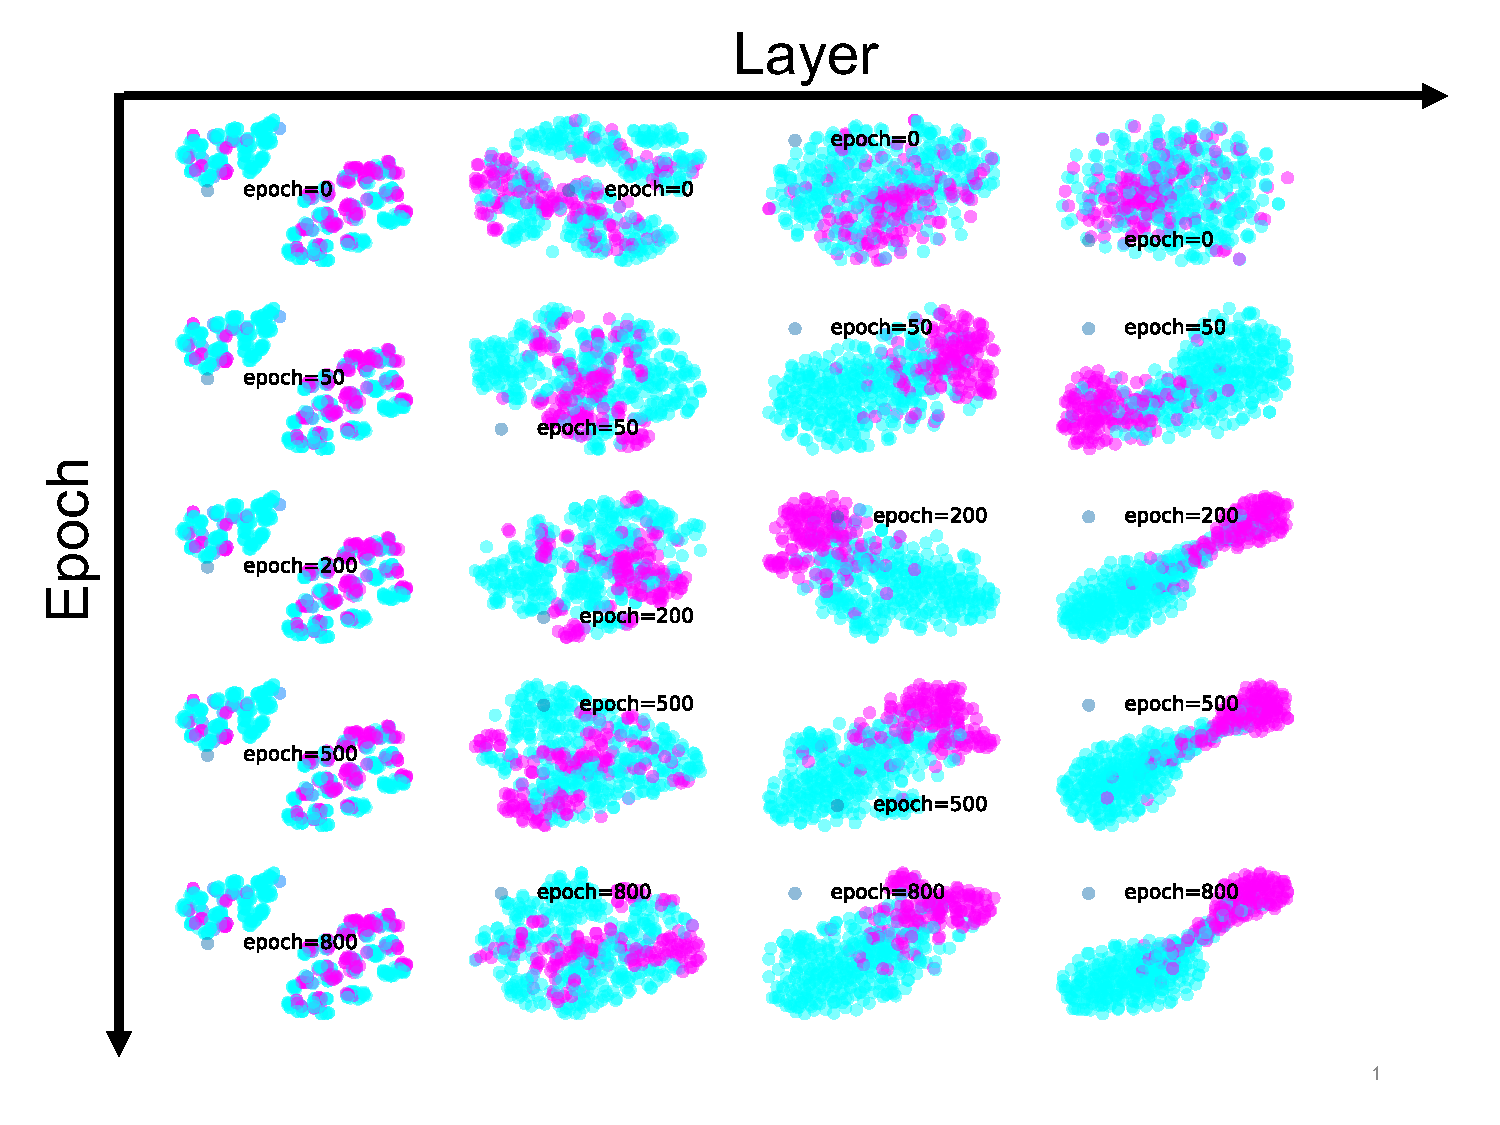
\includegraphics[width=8cm]{neural_networks/images/rep_learning}}; }] (Xp) at (3,3) {};}
\end{tikzpicture}

\end{frame}
%
\begin{frame}[t]{Conclusions}
In summary:
\vspace{1cm}
\pause{}
\begin{enumerate}
	\item Neural network models provide model complexity `on tap'\pause{}
	\item Backpropagation allows easy access to derivatives  \pause{}
	\item We can understand neural networks as automatic feature selection/transformation, followed by linear regression
\end{enumerate}

\end{frame}
%
\begin{frame}{ANN example}
jupyter notebook: \url{github.com/jpjanet/ML-chem-workshop/blob/master/notebooks/ANN.ipynb}
\end{frame}